\documentclass[conference]{IEEEtran}
\IEEEoverridecommandlockouts
% The preceding line is only needed to identify funding in the first footnote. If that is unneeded, please comment it out.
\usepackage{cite}
\usepackage{amsmath,amssymb,amsfonts}
\usepackage{algorithmic}
\usepackage{graphicx}
\usepackage{textcomp}
\usepackage{xcolor}
\usepackage{float}
\usepackage{stfloats}
\usepackage[backend=bibtex]{biblatex}
\addbibresource{References.bib}

\usepackage{listings}
\usepackage{xcolor}
\usepackage{caption}
\usepackage{booktabs}
\lstset{
  basicstyle=\ttfamily\footnotesize,
  backgroundcolor=\color{gray!10},
  frame=single,
  breaklines=true
}

\usepackage{tabularx}
\usepackage{adjustbox}


\def\BibTeX{{\rm B\kern-.05em{\sc i\kern-.025em b}\kern-.08em
    T\kern-.1667em\lower.7ex\hbox{E}\kern-.125emX}}
\begin{document}

\title{ Dynamic Sporadic Server\\

}

\author{\IEEEauthorblockN{ Moiz Zaheer Malik}
\IEEEauthorblockA{\textit{ B.Eng. Electronic Engineering} \\
\textit{Hochschule Hamm-Lippstadt}\\
Lippstadt, Germany \\
moiz-zaheer.malik@stud.hshl.de}

}

\maketitle

\begin{abstract}
In real-time systems, where tasks have different levels of critical importance, it is essential to serve aperiodic (irregular, event-driven) tasks while ensuring that the deadlines of high-priority periodic tasks are not violated. The Dynamic Sporadic Server (DSS) is a scheduling method designed for Earliest Deadline First (EDF) systems that addresses this problem. 

DSS is defined by a period  $T_s$ and a budget $C_s$, but unlike traditional sporadic servers, it does not restore the full budget at every period. Instead, when an aperiodic task arrives, DSS assigns it a deadline and restores only the amount of budget that was actually used. This approach allows the processor to reach full (100 percent) utilization while ensuring that all deadlines are still met. DSS improves the response time of aperiodic tasks without compromising the guarantees of periodic tasks.

Originally introduced by Spuri and Buttazzo\cite{spuri1994efficient}, DSS has been widely studied for its efficiency in managing mixed task sets under EDF scheduling. This report reviews the theory behind DSS, describes its operation (including budget management), highlights its advantages over traditional methods, and discusses potential application areas.
 
\end{abstract}

\section{Introduction}

Real time system often mix periodic tasks (reccurring tasks with fixed periods and deadlines) and aperiodic/sporadic tasks (tasks which arrive unpredictavly), for example interrupts or user request) And to ensure that the aperiodic tasks recive their service on time without causing problem to any aperiodic tasks to miss their deadlines is a majr challeng\cite{laplante2011real}. 

A common solution is to use Server Abstraction it is a concept used in real time systems to mannage how and when tasks (especially aperiodic or sporadic) are executed. Such as Polling Server, Deferrable server, and sporadic servers. The sporadic servers, introduced by Sprunt et al\cite{sprunt1989aperiodic}, assigns a fixed priorarity (typically through Tate Monotonic) to the server and provides a budget $C_s$ every period $T_s$. This allows aperiodic tasks to be executed with limited interference to hard real time tasks. However, under staticprority scheduling the processor often cannot be fully utilized, unused server budget might be wasted or caused complex analysis.

with dynamic scheduling (EDF) higher utilization can be achived. Dynamic priority server as shifted the sporadic server concept to (EDF). In particular, spuri and Buttazzo proposed the Dynamic Sporadic Server (DSS)\cite{spuri1994efficient}. Dss is characterized by a server period $T_s$ and capacity $C_s$ (the maximum aperiodic budget)\cite{buttazzo2011hard}. Unlike SS, DSS does not refill or replenish $C_s$ fully at each period start. Insted, the server's deadline and replenishment events are set dynamiclly whenever aperiodic work arrives or is consumed\cite{spuri1994efficient}. This allowes DSS to adaptivly use idle time for aperiodic tasks and to achive 100 percent CPU utilization. 

But the most important requirment is that under EDF schedule, the sum of the utilization of periodic tasks ($U_p$)\cite{buttazzo2011hard} plus the utilization of DSS ($U_s = C_s/T_s$)\cite{buttazzo2011hard} must satisfy In order to meet all deadlines\cite{spuri1994efficient}. 

\[
U_p + U_s \leq 1
   \ \cite{buttazzo2011hard} \]
   
Just like EDDF alone, DSS with EDF still allows 00 percent Cpu usage, so periodic tasks dont lose processing time. Unlike EDF, a fixed priority sporadic server cant fully use the CPU unless more complex analysis is done\cite{spuri1994efficient}.
   
\section{BACKGROUND: PERIODIC AND APERIODIC TASKS; EDF}
\textbf{Periodic task:} A periodic task $\tau_i$ generates tasks again and again, each job needs exeution time $C_i$ and must finish by a deadline $D_i$ after its arrival. commonly, $D_i = T_i$ (Deadline is equal to Period). The total Utilization of the periodic task is 

\[
U_p = \sum_i \left( \frac{C_i}{T_i} \right)
\ \cite{buttazzo2011hard} \]

based on the study by Liu and Layland\cite{liu1973scheduling}, The EDF algorithm can successfully schedule any set of periodic task (where deadlines are equal to periods) if and only if 

\[
U_p \leq 1
\ \cite{buttazzo2011hard} \]

\textbf{Aperiodic tasks:} More genral then sporadic, aperiodic tasks include all kind of arrivals, even the ones not allowed under sporadic rules. Aperiodic tasks can be unpridictable, they ussally have soft deadlines, which means they can somtimes miss ther deadlines. To measure how much CPU they need, we can look at their average or maximum load $U_a$. And the main goal of it is to serve these tasks quickly without effecting periodic tasks that have strict dedlines\cite{buttazzo2011hard}

\textbf{sporadic task:} Is a task comes at random times but with a rule there must be minimum gap (period)$T_s$ between two jobs. each job needs some time to run and execut $C_s$. Even though the job arive at irregularly, this minnimum gap helps to keep things under control. Because of this sporadic tasks are seen as simpler kind of periodic tasks with more flexible timing.\cite{buttazzo2011hard}.

\textbf{EDF Scheduling:}  Under EDF, tasks are assigned dynamic priorities equal to their absalut deadline (Earliest dealine = Highest ppriority). The EDF schedulability criterion rule workes with both periodic and aperodic tasks but only when tasks are treated like sporadic tasks with deadlines\cite{spuri1994efficient, buttazzo2011hard}.

However, simpl qeueing all periodic tasks under EDF can still cause problems for periodic tasks. Therefore server algorithms are used to controle how much CPU the aperiodic workload can use, effectively reserving bandwidth for aperiodic server\cite{buttazzo2011hard}. DSS is one such server, whch is used in EDF based system\cite{buttazzo2011hard}.

\section{SPORADIC AND DYNAMIC SERVERS}


\begin{figure*}
    \centering
    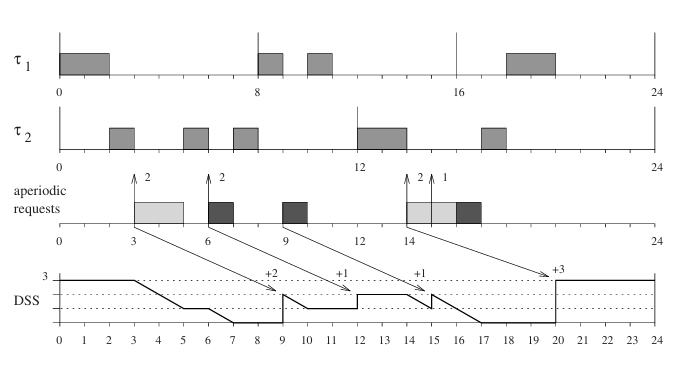
\includegraphics[width=0.8\linewidth]{Dynamic Sporadic Server example.jpeg}
    \caption{Dynamic Sporadic Server example \cite{buttazzo2011hard}}
    \label{fig:enter-label}
\end{figure*}



\subsection{The Sporadic Server (SS)} 

Before DSS, Sporadic server (SS) was used initially for fixed priority scheduling\cite{buttazzo2011hard}. The parameters of sporadic server are ($T_s$,$C_s$), Its rule is When an aperiodic task arrives and the serevr has avilable capacity, the server executes that job at high priority as long as it has budget. after consuming a amount of execution $U$, the server schedules a refil of $U$ after one period $T_S$\cite{buttazzo2011hard}.. The SS makes sure that the server uses as much of the the $C_s$ time in a period od $T_s$, ensuring pariodic tasks guarantees only if\cite{buttazzo2011hard}

\[
U_p + \frac{C_s}{T_s} \leq 1
\ \cite{buttazzo2011hard} \]

Where $U_p$ is the utilization of periodic taasks. However, in SS the serverperiority is fixed, making it not directly suitable for EDF system\cite{buttazzo2011hard}.

\subsection{The Dynamic Sporadic Server (DSS)}
The Dynamic Sporadic server (DSS) modifies the sporadic server (SS) for EDF Scheduling\cite{spuri1994efficient}.
Like SS, DSS has a server period $T_s$ and a Capacity $C_s$, DSS has dynamic deadlines rather than a fixed priority. the server the server behaves like EDF task whose deadline is recalculated at runtime when ever it begins servicing an aperiodic task. it budget does not resets simply at $T_s$, insted it's only consumed portions are recharged after $T_s$ units\cite{spuri1994efficient,buttazzo2011hard}.

The DSS behaves in the following way,
\textbf{Initialization:} The server starts with full budget $C_s$. No deadline $d_s$ is set until the first aperiodic job arives\cite{spuri1994efficient,buttazzo2011hard}.

\textbf{Activation:} When an aperiodic task arrives aat time $t_A$ and the server is idle with available budget $>0$, the server sets its current deadline $d_s$ = $t_A$ + $T_s$\cite{spuri1994efficient} and schedules its next refil at $R_T$ = $d_s$\cite{spuri1994efficient}. The server immediatly becomes the heighest priority EDF task and begins executing aperiodic ask. All aperiodic taskin that busy interval share the same deadline $d_s$\cite{spuri1994efficient}.

\textbf{Execution:} The server executes, deducting from its remaining capacity as it runs aperiodic tasks. If the aperiodic workload finishes before the udget is exhausted, the server waits with leftover budget. If more tasks arrive while budget remain, they are queued but served under the same deadline\cite{spuri1994efficient}. 

\textbf{Budget Exhaustion or Job Completion:} When capacity is exhausted or the last pending task finishes at time $t_I$, the server computes how much budget $u$ was consumed since $t_A$ and schedules a refil of amount $u$ at time $R_t$. if pending tasks remain after exhaustion, they are paused until the refil\cite{sprunt1989aperiodic, spuri1994efficient} 

\textbf{Next Activation:} afetr refil at every $R_T$, if there are tasks pending the server repeates the activation step, it sets a new deadline $d_s$ = $R_T$ + $T_s$ and executes again. 

These rules ensure ever consumes more the the $C_s$ time in any period $T_s$\cite{spuri1994efficient,buttazzo2011hard}. Thus DSS behaves like aperiodic task under EDF. The schhedulability condition for mixing DSS with periodic task is\cite{buttazzo2011hard}
\[
U_p + U_s = \sum_i \frac{C_i}{T_i} + \frac{C_s}{T_s} \leq 1
\ \cite{buttazzo2011hard, spuri1994efficient} \]

Where $U_p$ is the utilization of periodic task and $U_s$ = $C_s$/$T_s$ is servers utilization\cite{buttazzo2011hard}.

\textbf{Mathematical Formulation:} Formally, it can be shown (Lemma and Theorem in~\cite{spuri1994efficient}) that in any busy interval of length $\Delta$, the server executes at most $C_s$ time per $T_s$ window. 
Thus, DSS achieves full utilization in EDF-based systems, as long as $U_p + U_s \leq 1$  \cite{buttazzo2011hard}.

This means the dynamic sporadic server behaves like a periodic task when it comes to CPU usage any interval of the length equal to its period $T_s$, it will neever see more than its budget $C_s$. so if the utilization from all the periodic tasks plus the DSS remains at or below 100 percent all dadlines can be met. this schedulability condition has been formally proven to be both necessary and sufficient for EDF system using DSS \cite{buttazzo2011hard, spuri1994efficient}.

\begin{figure}
    \centering
    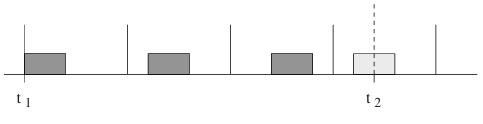
\includegraphics[width=1\linewidth]{image.png}
    \caption{Computational demand of a periodic task in [t1,t2] \cite{buttazzo2011hard}.}
    \label{fig:enter-label}
\end{figure}

\section{Dynamic Sporadic Server Simulation}


From the Fig 1 Dynamic sporadic example from \cite{buttazzo2011hard}, it shows two periodic tasks $\tau_1$ and $\tau_2$ along with a Dynamic Sporadic Server (DSS) that Will work on serving incoming aperiodic requests. task $\tau_1$ has period $P_1=8$ and execution time $C_1=2$, while $\tau_2$ has $P_2=12$ and $C_2=3$. The Dynamic Sporadic Server (DSS) has a period $T_s=6$ and capacity $C_s=3$. aperiodic tasks arrives at spacific times (for example at $t=3,6,9,\dots$ with different execution demands) and are inlined for service by DSS. The scheduler uses earliest deadline first (EDF) policy. \cite{buttazzo2011hard}.

the DSS logic follows the standard rules: its budget is initialized to  $C_s$ and is refilled one period after being activated for eachtime\cite{buttazzo2011hard}. whenever a new aperiodic requiest arrives and the server is idle with remaining budget, the server becomes activated, and its deadline is set to (current time + $T_s$)\cite{buttazzo2011hard}) while active, the server executes as long as there is pending apepriodic work and budget, each execution unit decrements both the server's remaining capacity and activity aperiodic job's remaing work. and if the server finises it sbudget and complet all iofits pending tasks, aperiodic tasks. it becomes inactive after that and schedules it s consumed budget to be refilled at the previously assigned deadline \cite{buttazzo2011hard}.

\section{DSS-Based UPPAAL Model Simulation}


\begin{figure*}
    \centering
    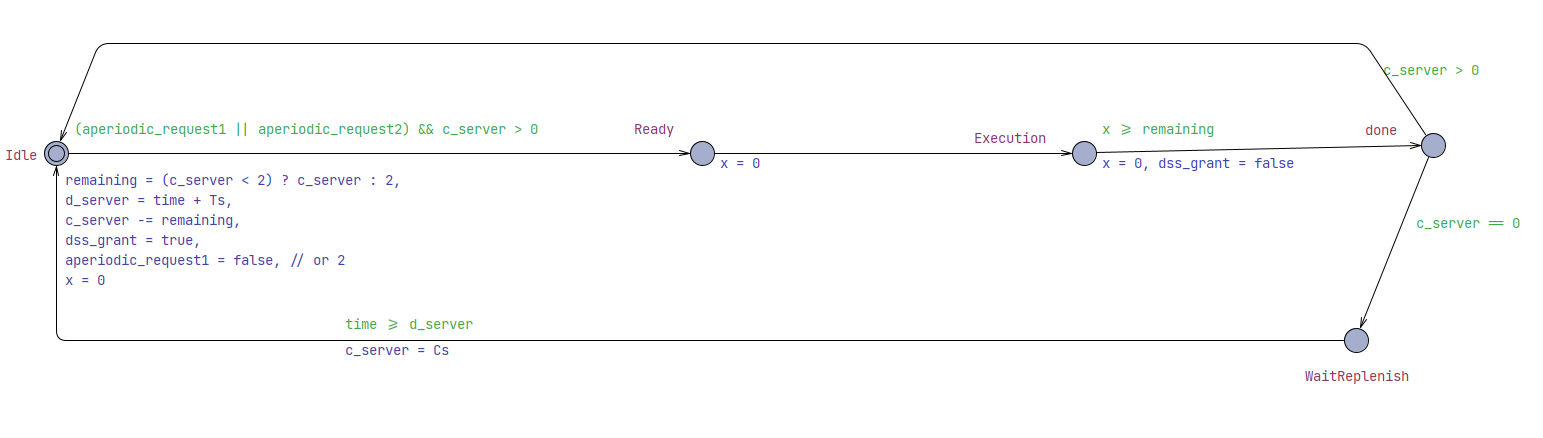
\includegraphics[width=1\linewidth]{DSS Server.png}
    \caption{DSS server}
    \end{figure*}

\begin{figure*}
    \centering
    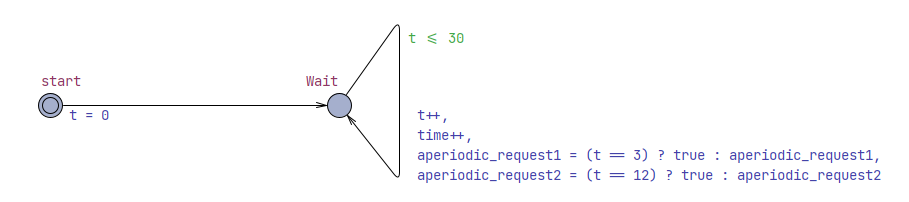
\includegraphics[width=1\linewidth]{Controller.png}
    \caption{Controller}
    \label{fig:enter-label}
\end{figure*}
 
In this seminar, I'am presenting a dynamic sporadic server (DSS) simulation using UPPAAL. the main goal was to show how DSS scheduling works and handels aperiodic tasks without intrupting and disturbing the Perioidic tasks, which is very important in real times systems. The simulation i made includes two pperiodic tasks, two aperiodic tasks, DSS server, and a controller which acts as the envirnment.

the periodic task are designed tp run at fixed intervals. \textbf{PT1} has a perioid of 8 time units and executes for 2 time unites, while \textbf{PT2} has a shorter perioid 5 unites and it and executes for 1 time unit. Each periodic tasks move through four states: \textit{Idle}, \textit{Ready}, \textit{Execution}, and \textit{Done}. When the period expires, the task moves to  \textbf{READY}, then executes for its set time, and then goes to execute \textbf{DONE} before resetting. 

for Aperiodic part, I again includeed two tasks that are not triggered by time but by events. \textbf{APT1} runs for 2 unites and is triggered by the controller at time $t=3$. \textbf{APT2} runs for 3 unites and is triggered at $t = 12$. however, these tasks can't just start in their own. they must be allowed by the DSS server through a signal called \textbf{dss\_grant}. this means that even if a request comes in, the task will only run if the DSS says it can.

The \textbf{DSS\_Server} is the key part of the whole model. It manages when and aperiodic task can execute. The capacity of the server is $C_s$ of 3 units, which means it can be spend up to 3 units on aperiodic task before it refill. the period of replenishment period $T_s$ is 6 units. the DSS goes through sevral states, \textit{Idle} (watching for new requests), \textit{Ready} (when it decides to grant access), \textit{Execution} (running an aperiodic task), \textit{Done} (after the task finishes), and \textit{WaitReplenish} (when it has no capacity and is waiting to refill). It keeps track of how much capacity it has and also remembers when to refill again. with \textbf{d\_server}.

The \textbf{Controller} in the model is a simple component that simulates the enviourment. It keeps track of time and triggers the aperiodic task requests at specific points. in my simulation, it sets \textbf{aperiodic\_request1 = true} at $t = 3$ and \textbf{aperiodic\-request2 = true} at $t = 12$. 

When the simulator runs, both periodic tasks start in \textbf{Idle}. at time $t = 3$, When the first aperiodic task arives it is then triggered by the  controller. scince DSS has full capacity at the start, it grants permission, and \textbf{AperiodicTask1} execute, then the first replenishment time and the server is. Scince $d_s$ is the earliest deadline first, the highest priority shifts toward DSS task in th esystem and the request gets served unti completion\cite{buttazzo2011hard}. This reduces the the servers capacity from 3 time units to 2 units then again the periodic tasks continue executing according to their periods \textbf{PeriodicTask2} runs at $t = 5$ and \textbf{PeriodicTask1} at $t = 8$. At $t = 12$, the controller sends the second aperiodic request\cite{buttazzo2011hard}. Now depending how much capacity the DSS has left, it will run the second task for that period and after he refil it again runs it\cite{buttazzo2011hard}.

The simulation clearly shows how DSS works and how it serves the aperiodic tasks without intrupting the periodic tasks. The DSS carefully tracks how much capacity is used and refills only after the defined period. This method ensures that periodic tasks always get priority and deadlines are not missed, while still giving space to aperiodic tasks when possible. I believe this model demonstrates the concept in a simple but effective way, and helps to understand real time scheduling more practically.



\section{Comparison with Other Servers}

Table~\ref{tab:servers} shows the comparesion of the key features of Polling,Deferrable,sporadic and dynamic sporadic server. polling server operate under fixed priority scheduling and resets it budget after each period regardless of use \cite{sprunt1989aperiodic}. Deferrable servers also run at high prority but carry their unused capacit till the end of the periode \cite{buttazzo2011hard}. The classic Sporadic server fro Ratemonotonic schedulling only replenishes only the portion of their buddget that was actually used \cite{sprunt1989aperiodic}.


\begin{table}[ht]
\centering
\renewcommand{\arraystretch}{1.1} % Optional: add some vertical spacing
\begin{tabularx}{\columnwidth}{l|X|X|X|X}
\textbf{Feature} & \textbf{Polling} & \textbf{Deferrable} & \textbf{Sporadic} & \textbf{DSS} \\
\hline
Scheduling & Fixed-priority (RM) & Fixed-priority (RM) & Fixed-priority (RM) & Dynamic (EDF) \\\\
Priority & Highest static & Highest static & Static (RM) & Dynamic (deadline $t+T_s$) \\\\
Replenishment & Periodic full & Periodic full & On-demand & On-demand \\\\
Unused Budget & Lost if unused & Carried to period end & Carried to next period & Reused flexibly \\\\
Utilization & Often suboptimal & Improved response & Moderate & Full (up to 100\%) \\\\
\end{tabularx}
\caption{Comparison of Aperiodic Servers}
\label{tab:servers}
\end{table}


Because of the EDF and its flexible budget useage Dynamic sporadic server stands apart from others. In practice, DSS provides the responsiveness of a high priority server without leaving CPU time idle when aperiodic demand is present  \cite{buttazzo2011hard, laplante2011real}.

\section{Applications and Use Cases}

Dynamic Sporadic Servers (DSS) are well-suited to systems that must mix hard real-time periodic tasks with unpredictable aperiodic workloads. Typical examples include automotive ECUs, robotic controllers, avionics systems, embedded Linux platforms, multimedia devices, and medical equipment.

For instance, an automotive braking controller may have a periodic speed-monitoring task and a sporadic braking-request task \cite{spuri1994efficient}. In such domains, DSS provides a reserved capacity for aperiodic jobs without violating hard deadlines of periodic jobs.

In robotics, a servo loop may run at a fixed rate while sensor or vision processing tasks arrive unpredictably. DSS can absorb these aperiodic jobs using its time-varying deadline mechanism (e.g., “ties are always resolved in favor of the server”) \cite{buttazzo2011hard, spuri1994efficient}, improving responsiveness without jeopardizing safety-critical loops.

Similarly, avionics flight computers often interleave periodic control tasks (e.g., stabilization) with aperiodic ones (e.g., communication, diagnostics). In multimedia systems, the Linux \texttt{SCHED\_DEADLINE} scheduler uses a variant of DSS (Constant Bandwidth Server) to serve aperiodic workloads (network packets, user interactions) alongside real-time tasks \cite{buttazzo2011hard, spuri1994efficient}.

In medical systems such as implantable monitors or patient alarms, DSS can isolate life-critical periodic sensing from sporadic events like logging or alarms.

\begin{itemize}
    \item \textbf{Automotive ECUs:} DSS allocates a fixed budget $C_s$ per period $T_s$ to event-driven aperiodic tasks without delaying periodic engine control jobs \cite{spuri1994efficient}.
    \item \textbf{Robotics and Control:} DSS enables mixing real-time servo loops with irregular processing (vision/path planning) while meeting EDF feasibility conditions \cite{buttazzo2011hard}.
    \item \textbf{Avionics:} DSS helps meet deadlines for both periodic sensor/actuator cycles and asynchronous diagnostics.
    \item \textbf{Embedded Linux \& Multimedia:} DSS variants like CBS are used in Linux for EDF-based scheduling of sporadic user interactions or audio/video streams \cite{buttazzo2011hard}.
    \item \textbf{Medical Systems:} DSS ensures timely response to alarms while maintaining guaranteed periodic monitoring rates.
\end{itemize}

DSS offers strong temporal isolation: aperiodic tasks are treated like a periodic task with utilization $U_s = C_s / T_s$. Spuri and Buttazzo showed that if $U_p + U_s \leq 1$, all EDF deadlines will be met \cite{spuri1994efficient, buttazzo2011hard}.

\section{Limitations and Practical Considerations}

Implementing DSS involves non-trivial complexity. The operating system must manage a dynamic deadline and a replenishable budget. Each aperiodic job arrival or execution requires updating the deadline and tracking consumed capacity \cite{buttazzo2011hard, spuri1994efficient}. This includes scheduling a replenishment for any consumed portion after $T_s$ time units.

Whenever an aperiodic job executes, it inherits the server’s deadline and may preempt periodic jobs. This makes DSS more complex than simple polling or deferrable servers \cite{spuri1994efficient,laplante2011real, buttazzo2011hard}.

In systems using fixed-priority scheduling (e.g., Rate Monotonic), DSS cannot be directly implemented. It relies on EDF for dynamic prioritization. While real-time Linux and some RTOSes support CBS/DSS, integration still requires modifying scheduler internals.

There is also an overhead trade-off: smaller $T_s$ reduces latency but increases context switching. A short $T_s$ means smaller budgets $C_s$, which may lead to queue buildup. Conversely, large $T_s$ values reduce overhead but delay service to aperiodic jobs \cite{spuri1994efficient,laplante2011real}.

Heavy aperiodic workloads can overwhelm the server. If job arrivals exceed $U_s$, delays increase sharply. Worst-case latency occurs when jobs arrive just after budget exhaustion. System designers must choose $T_s$ and $C_s$ carefully to balance responsiveness with feasibility.

Corner cases also matter. If a server and a periodic job become ready at the same time, tie-breaking policies must prioritize the server \cite{buttazzo2011hard, spuri1994efficient}. Priority inheritance protocols are needed to avoid deadlocks when tasks share resources. In multicore systems, sharing the server budget across cores further complicates scheduling.

In summary, DSS offers predictability but requires careful implementation and tuning.

\vspace{1em}
\section{Conclusion}

The Dynamic Sporadic Server is a powerful scheduling mechanism that extends EDF by offering guaranteed bandwidth to aperiodic tasks. By dynamically assigning deadlines and replenishing only the used capacity, DSS achieves efficient processor utilization while respecting hard deadlines for periodic tasks \cite{spuri1994efficient, buttazzo2011hard}.

Its strengths include:
\begin{itemize}
    \item Strong temporal isolation and bandwidth reservation.
    \item High responsiveness to aperiodic jobs.
    \item Full utilization up to 100\% under EDF schedulability bounds.
\end{itemize}

DSS is particularly beneficial in mixed-criticality real-time systems such as automotive, avionics, robotics, and embedded Linux environments. Compared to simpler servers, it provides better control and responsiveness, especially under unpredictable workloads.

Looking forward, DSS can be enhanced through variants like the Constant Bandwidth Server (CBS), integration with priority-inheritance protocols, and adaptations for multicore platforms \cite{laplante2011real}. Future research may also explore hybrid EDF-fixed priority schemes and virtualization-aware servers.

In conclusion, DSS remains a relevant and effective solution for real-time systems that require dynamic, predictable aperiodic task management


\printbibliography


\vspace{12pt}
\color{red}


\end{document}
